\documentclass[12pt]{report}
\usepackage[utf8]{inputenc}
\usepackage{graphicx} 
\usepackage{hyperref}
\graphicspath{{images/}}
\usepackage[a4paper,width=150mm,top=25mm,bottom=25mm]{geometry}
\usepackage{fancyhdr}
\pagestyle{fancy}
\fancyhead{}
\fancyhead[R]{sense2vec}
\fancyhead[L]{\chaptername~\thechapter}
\fancyfoot{}
\fancyfoot[R]{\thepage}
\fancyfoot[L]{Shane Smullen}
\usepackage{caption}
\usepackage{subcaption}
\usepackage{float}

\title{
    {Sense2Vec: Investigating the Advantage of Introducing Part of Speech Tagging When Training Word Embeddings}\\
    {\large Maynooth University}\\
    {
\includegraphics[scale=0.5]{university}}
}
\author{Shane Smullen}
\date{April 2020}

\begin{document}

\maketitle

\begin{abstract}
Many methods for producing word embeddings have been developed but one project considered the standard, Word2Vec is able to extract context and give the illusion of knowledge when trained on a corpus of text. However it is not without its pitfalls, when investigating Word2Vec's ability to group verbs it does not produce the same level of quality as with noun embeddings. The Sense2Vec project introduces part of speech tagging to the training process allowing for a more refined level of context to be obtained. When investigating verb embeddings specifically a greater relationship was found between verb tenses than originally produced by Word2Vec. Also by making a distinction between words that may be considered a noun or a verb depending on context, a more refined list of similar embeddings is produced.
\end{abstract}

\tableofcontents

\chapter{Introduction and Problem Overview}
\section{Natural Language Processing (NLP)}
The task of processing human language is one that is complex and is a combination of many areas of research including speech recognition, language generation and understanding to name a few. All developments in this area require the processing and analysis of large amounts of ordinary human language known as natural language. The area of NLP has importance many current technologies from obtaining personalised recommendations online to speech recognition to create text-to-speech systems. While it is clear in recent years huge developments have been made in this area and research in the field of natural language has been around for almost as long as language itself, the task of processing this natural language is still a non trivial problem. Firstly there is the problem of natural language itself, the first hurdle is syntax. This defines the formal grammar of the language, the part of speech of the words in a sentence example verb, noun adjective etc. Next is semantics which is based on the meaning of words in a sentence which is particularly important in translation, where it is important to identify the names of places and people in the English language these are capitalised other languages have different semantics for this. Both syntax and semantics both have more tasks to overcome to fully understand and describe the natural language they belong to. Chapter 2 presents a more in depth analysis of how these tasks are used in the area of natural language processing. 

With the sharp increase in the availability of data in recent years the possibility to develop more intelligent systems has drawn the attention of many researchers and companies. However the processing of this large amount of language data is now a new problem alongside the understanding of the language. While many methods have existed for years for the processing of this data, these methods were originally created before this abundance of language data was available and as such are not suited to processing the size now available. A gap was created as huge amounts of data were now available with few ways to process it, the introduction of machine learning was the plan to solve this issue. Many current solutions use this method, examples of such include the extraction of events for incoming emails, auto-correction of text and many more.

\section{Problem Overview}
The solution presented in chapter 3 will focus on the syntax and semantics of NLP, looking at the parts-of-speech in the English language and the similarity between them. While this similarity will investigate on all parts-of-speech there will be a focus on verbs and pronouns, as there appears to be little research done in this field. A new method for investigating this similarity between words has recently appeared, with this new method it is possible to compute the similarity between verbs and pronouns. This new method will be bench marked against older methods, the results of which will be presented in chapter 4, with an analysis of these comparisons presented in chapter 5.

Within chapter 4 a broad selection of results will be presented, these results will compare three technologies, Word2vec, Sense2Vec and WordNet. As discussed above there is now an abundance of data which can be analysed and used for modeling. In chapter 3 where this data was obtained and how it will be processed will be discussed. The training process will be shown in detail and improvements to this process will be presented. Any conclusions obtained from these results will show if any changes to previous technologies are positive, negative or unchanged. Not only is it important to highlight the positive and negatives of using these technologies, it is also key to validate the results produced and show a distinctive difference between the technologies. The methods used to validate the results and the technologies used will demonstrated at the end of chapter 2.

\chapter{Background}
\section{Current Implementations}
The current de facto standard for representing words in vector space is Word2vec. In this vector space each vector corresponds to a single word, these word vectors are contained in multidimensional space with their length and direction altered based on the words use in a given corpus. The creation of these vectors is a multi step process:
\begin{enumerate}
    \item Data Preparation - Define corpus, clean, normalise and tokenise words
    \item Hyper parameters - Learning rate, epochs, window size, embedding size
    \item Generate Training Data - Build vocabulary, one-hot encoding for words, build dictionaries that map id to word and vice versa
    \item Model Training - Pass encoded words through forward pass, calculate error rate, adjust weights using back propagation and compute loss
    \item Inference - Get word vector and find similar words
    \item Further improvements - Speeding up training time with Skip-gram Negative Sampling (SGNS) and Hierarchical Softmax
\end{enumerate}

\noindent
Word2vec can be trained in two ways Continuous Bag-Of-Words (CBOW) or continuous Skip-gram (SG). CBOW will attempt to guess the output; a single word from surrounding words and generally is faster to train. While SG will attempt to guess context words from a single word and tends to work better when only a smaller corpus is available. This choice must be made at the begining of training and generally two models are created one for each method. \cite{Mikolov} For more examples and distinctions between the two see Appendix A.

Word2vec has many strong use cases with a focus in information retrieval and knowledge discovery. One such example is where Word2vec was used to identify new chemical compounds based on specific properties. In this paper the training corpus was approximately 3.3 million abstracts from 1000 different journals. By looking at relations between different compounds using analogies learned during the training process. In this case Word2vec was integral in the training process, chemical formulae were included in normalised form and trained using skip-gram. The end result was the ability to enter a normalised formulae with the SG model returning a list of context words some of which being a property of the supplied compound such as thin, magnetic etc. \cite{Tshitoyan}

\section{Vector Combinations}
One of the strengths of Word2Vec is the ability to subtract two vectors and add the result to a third, allowing for another form of relationship between word vectors to appear. This concept is one of the best examples to show how Word2Vec can give the illusion that semantic understanding is built into the Word2Vec model. This concept was introduced in the original Word2vec paper by employees at Google in 2013 and includes some promising results.

\begin{figure}[h]
    \centering
    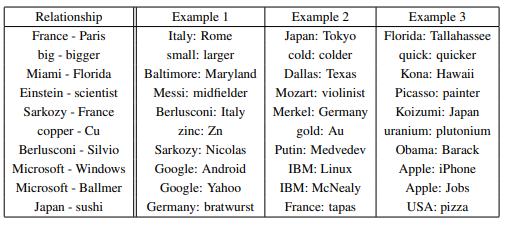
\includegraphics[width=\textwidth]{images/learned_relationships}
    \caption{Word pair relationships}
    \label{fig:table_relations}
\end{figure}

\noindent
In figure ~\ref{fig:table_relations} the subtraction vectors appear in the left column and the addition vector is listed before the colon in each subsequent column. The resulting vector is then given, for example in the first row Paris is subtracted from France and Italy is added giving the result of Rome. In the original creation of Word2Vec this process was correct approximately 60\% of the time. \cite{Mikolova} It may be easy to say in figure 2 that the model has some sort of understanding of language as it provides logical results in figure ~\ref{fig:table_relations} however it is important to note that this understanding is extracted embedded \textit{meaning} within the corpus. Therefore this extraction of meaning may be biased based on the supplied corpus, and example of which was used to show the possibility that Amazons AI recruiting tool formed a bias against women. This bias appears to have formed from the data used and not from the model \cite{Caliskan}, in this paper Word2vec was used in combination with Glove. Glove, created in Stanford can be used to identify structure within the generated vector space and in this case was used to identify the bias embedded within the corpus. \cite{Pennington}

\section{Cosine Similarity}
 The representation of words as vectors can give the appearance of meaning in text using methods such as Word2Vec. This meaning can appear due to the way Word2Vec represents words vectors in high dimensional space. When the Word2Vec model is queried with two input vectors the vectors are found in the model and by calculating the cosine similarity between these two vectors a value between zero and one is obtained. Naturally the vector representation of words such as car and wall will have a value close to zero while wall and house will produce a value closer to one. This ability to obtain a value between zero and one for how similar two words allows for the extraction of basic meaning from text. 
 
 The cosine similarity allows for the abstraction of the length of the word vectors and instead will focus on the angle between said vectors. This idea overcomes the general approach of counting the most common words to tell if a document is similar or in the case when investigating words counting the common letters. This ability to ignore magnitude and focus on angles in multidimensional space allows for more meaningful relations to be found.
 
 \begin{figure}[h]
    \centering
    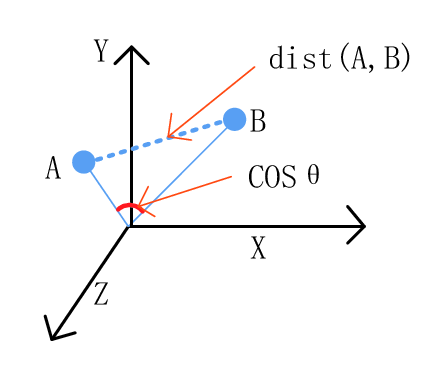
\includegraphics[width=.55\textwidth]{images/cosine_sim.png}
    \caption{Cosine similarity use case}
    \label{fig:cosine_vectors}
\end{figure}

\noindent
As seen in figure \ref{fig:cosine_vectors} \cite{Wang1} two vectors are separated by some distance which is a combination of their length and the angle between them. By using the cosine angle between A and B and avoiding length the definition of \textit{closest vector} changes. As A or B appears more frequently in the corpus and in turn increases the length of the vector the same cosine angle will hold. When a word appears in different contexts, its vector gets pulled or pushed in different directions changing the cosine angle. The final vector then represents some sort of weighted average over the various contexts. 

\section{Word Depth} 
The definition of word depth used here is in reference to semantic lexicons, these semantic lexicons are made up of entities. Each lexical entity is connected by semantic relations. In WordNet, entities with multiple meanings (synonymous) are grouped into what it calls synsets. WordNet is a lexical database project from Princeton University which includes four categories noun, verbs, adverbs and adjectives. When comparing noun and verb depth it is required to look at how WordNet data is organised into hierarchies. These hierarchies are created through the use of hypernyms. \textit{Y is a hypernym of X if every X is a (kind of) Y.} Noun hierarchies are far deeper than verb hierarchies.

This depth difference can disrupt matching when preforming similarity queries in WordNet. With nouns having a deeper tree of hypernyms than verbs, it is more likely when comparing similarity between nouns a higher value will be found. This problem of word depth extends to other methods also, when preforming cosine similarity queries in Word2vec a more diverse range of scores is found when using nouns as opposed to verbs. Another factor that affect these scores in Word2vec is the lack of part of speech tagging (POS) in Word2vec.

\section{Verb Group sets}
Grouping words based around a specific category is often a difficult task, with verbs defined as action words one such grouping is commonly used by information professionals. Bloom's Taxonomy is centered around learning objectives and is structured as a hierarchy containing six categories. Within each of these categories verbs are used to define the learning objective.

\begin{figure}[H]
\centering
  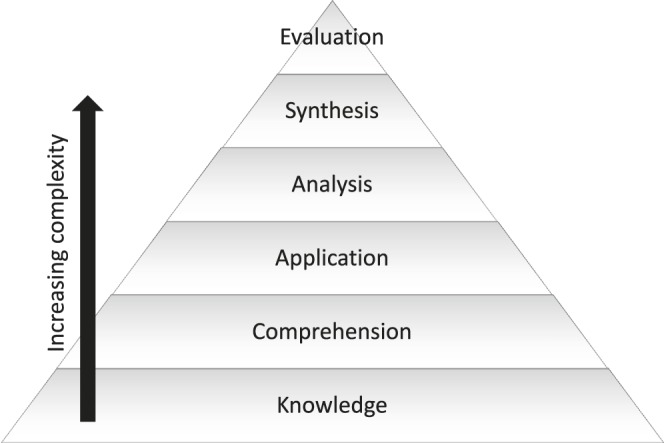
\includegraphics[width=.9\textwidth]{images/bloom.jpg}
  \caption{Bloom's Taxonomy}
  \label{fig:bloom}
\end{figure}

\noindent
By examining the verbs within each level it encourages instructors to think of learning objectives in behavioral terms to consider what the learner can do as a result of the instruction. \cite{Adams2015} Verbs within each category should have a high relational similarity as well as verbs between levels, with decreasing similarity the further the level away from the one being examined. As the complexity increases up the hierarchy actions or verbs within the evaluation category will require a much deeper understanding then those in the knowledge category.

\chapter{Problem Specification and Solution}
\section{Systems Used: Sense2Vec}
The Sense2Vec model is built on a previous method for learning continuous word embeddings known as Word2Vec. Sense2Vec introduces the idea of attaching word senses before beginning the training process this requires part of speech tagging each word in the corpus and is the costliest procedure in the training process. However, the introduction of POS tagging in the process allows a word to be predicted by its surrounding senses rather than by the surrounding words. In base Word2Vec the closest vectors to a supplied word can often be a mixture of proper nouns, verbs and nouns. When supplying the POS with word the query will return a cluster of vectors more relevant to how that word is used. When obtaining the cosine similarity for a proper noun and supplying the POS PROPN Sense2Vec will return vectors more relevant to the use of the noun, this is especially useful when a word can have multiple meanings for example “apple” this could refer to the PROPN of the company Apple or the NOUN apple. Here Sense2Vec is able to extract extra meaning from the word by incorporating the POS of the supplied word, when supplying the word “apple” to Word2Vec the model obtains the cosine similarity of the closest n vectors regardless of where in the sentence the word and the resulting vectors are used. With Sense2Vec a completely different cluster of vectors are obtained when the NOUN and the PROPN are queried resulting in relevant vectors based on the words usage. \cite{Trask2015}

Incorporating POS to obtain extra meaning becomes extremely useful when looking at word depth, as discussed before due to verbs having a much shallower word depth than nouns the meaning of the verb is difficult to extract when using a Word2Vec model. By introducing senses, it allows for the differentiation of a words usage and in turn produces more relevant vectors when using cosine similarity. A comparison of this extra meaning will be shown later in Chapter 4 Results, but one example would be the word “play” with the Word2Vec model there is no differentiation between the verb “to play” and the noun “a play”. Here the resulting n similar vectors would be a combination of both with the verb possibly getting more priority due to more usage than the noun depending on the corpus. Sense2vec removes this ambiguity by differentiating between the verb and the noun which has the result of removing the variable of how often the word is used in each context.

\section{Systems Used: Stanford NLP}
The first step in the training process requires POS tagging each word in the corpus this is the most expensive part of the training process for Sense2Vec. Perfect POS tagging would require constructing a parse tree for the corpus, see Appendix B for further discussion on this process.

However, with the recommendation for Sense2Vec to have a corpus of at least 1 billion words constructing a parse tree of this size for the full corpus would be unfeasible. The Sense2Vec project contains scripts parse and tag a supplied corpus which use the Spacy library made by the same team. This library is relatively new and contains extra features not required for POS tagging, Spacy was not designed as research software and would remove the option for flexibility in the future should it be used. For easier integration and future use of the training methods it was decided that the use of the Stanford NLP library would be used for POS tagging. Stanford NLP has a self-contained python library for which can be used for POS tagging and provides an official Python wrapper for accessing the Java Stanford CoreNLP Server, this allows for the construction of smaller batches of parse trees on segments of the corpus.

This required the rewriting of the original parse process developed by for Sense2Vec using Stanford NLP, once imported the pretrained English models can be downloaded and the pipeline created. This pipeline is what separates Spacy and Stanford, some important options can be configured when using this pipeline. One of which is the Processors option, here it is possible to add or remove processors depending on what is required. In this case the main processor used was the POSPrecessor, however Stanford NLP includes others which provide a more accurately tagged corpus and are required to use the above these include the following:

\begin{itemize}
  \item TokenizeProcessor for segmenting the document into sentences
  \item MWTProcessor for expanding multi-word tokens into multiple words
  \item LemmaProcessor to preform lemmatization of words for example the word "better" has "good" as its lemma.
\end{itemize}
More details on the processors used and the values for each can be found in Appendix E. Each of these processors contain a batch size this is the number of words processed in each batch in this case the default is 5000 and is dependent on the RAM of the computing device. This will be based on the GPU RAM if the use\_gpu is selected when creating the pipeline, in this case a gpu was not used for POS tagging this will be discussed further in the Parsing and POS Tagging section.

\section{Parsing and POS Tagging}
For a fair comparison between Word2Vec and Sense2Vec it was necessary to train both models on the same corpus in this case a corpus of the latest Wikipedia articles was used resulting in a corpus of just over 15GB. This corpus is supplied for public use from Wikipedia and is available online at https://dumps.wikimedia.org/enwiki/ this is a compressed xml file which requires extraction and parsing. The Gensim python library which is used later in training provides a WikiCorpus function for extraction and parsing of each article to text. Each article yields a token where each token was decoded using utf-8 and written to an output file. This wiki.txt output file obtained from WikiCorpusExtractor.py was then used to train both Word2Vec and Sense2Vec models used in Section 3.5 Extracting Results, this process is discussed further in Appendix D.

POS tagging is not required when training Word2Vec however this is what separates the two processes. As discussed earlier Stanford NLP is used when POS tagging the corpus this process is heavily dependent on the RAM of the computing machine and at default the number of words processed during each batch is 5000. With a corpus size of over 15GB it is not possible to load the full corpus into memory for processing as such an iterator is used to return single wiki articles for processing. This assumes the corpus is one document per line and tokens are separated by whitespace. Each line in the corpus is then converted to a doc object for processing by Stanford NLP, once complete the doc object contains sentences which contain words. The .text attribute can be called on this word object to obtain the text and more importantly the .upos attribute contain the universal part of speech tag for the word used in the sentence example NOUN, VERB etc. In cases where the line yielded by the iterator exceeded the memory limit set when creating the Stanford pipeline. The line is broken up into segments less than the size of the word limit and processed as above until the line is complete.

\section{Training}
The process of training for a Word2Vec model is more streamlined than the process for Sense2Vec, once again an iterator is used to obtain single articles from the corpus. This data is passed to the Gensim library containing the Word2Vec, here the min\_count was changed to 1 the training will ignore all words with a frequency less than this value. As discussed in section 2.1 Word2Vec can either use skip gram or CBOW this is decided during training using the sg parameter, in this case both a skip gram and a CBOW model was produced. With Sense2Vec the process of model training is more involved first requiring the input corpus to be POS tagged before any training begins. The bulk of the processing is done using GloVe another project from Stanford NLP. GloVe is designed capture as much as possible the meaning specified by the juxtaposition of two words, take for example “man” and “woman” in one case they can be placed into the category of human however they can also be considered opposites. \cite{Pennington} 

\begin{figure}[h]
    \centering
    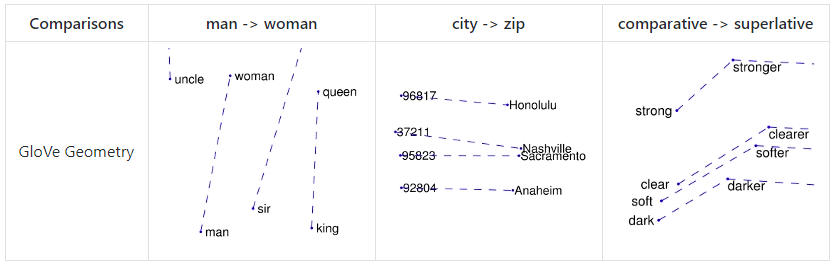
\includegraphics[scale=0.65]{images/GloVe.PNG}
    \caption{Learned Vector Representation}
    \label{fig:GloVe}
\end{figure}

\noindent
Before training can commence three files must be generated using GloVe: 
\begin{itemize}
  \item vocab.txt which stores a list of each unique word in the corpus and its number of occurrences
  \item cooccurrence.bin to store a co-occurrence matrix, which tabulates how frequently words co-occur with one another in the given corpus.
  \item cooccurrence.shuf.bin a shuffled version of the co-occurrence matrix above
\end{itemize}
This process has been completed already by the team behind Sense2Vec and they have supplied the necessary scripts for the GloVe training process. The use of these GloVe and these scripts do come with some caveats and the need for minor edits. GloVe requires the use of bash commands on a Linix system, these commands can however be called from Python itself. The scripts supplied by Sense2Vec use the implementation of f-Strings in Python3.7 in a few cases these commands are formatted incorrectly and require changing. Also of course a major downside to this process is if a Python version less than 3.7 was in use this would require some major changed to the code. Finally, one last script is used 05\_export.py this file loads the vectors file and the frequency file (vocab.txt) and generates a Sense2Vec component that can be loaded via Sense2Vec.from\_disk.

\section{Extracting Results}
Once the models for both Word2vec and Sense2Vec are obtained they can be loaded into memory when needed, both have functions for obtaining n number of cosine similar vectors. While it is a straightforward process to query the models one other benchmark is used against the two systems, WordNet allows the use of a path similarity value between two synsets. This process is somewhat cumbersome as the path similarity method must be called on one synset object passing the comparison synset object as an argument. As such a small wordnet\_similarity function was created to compare path similarity between two words. One major advantage of this is that WordNet itself contains POS tags for each synset and so a benchmark can be used against Sense2Vecs use of POS tagging.

Some of the results are used to highlight Sense2Vecs ability over Word2Vec and WordNet however as to avoid cherry picking results some randomness and statistical methods are used. The first of these methods involves two large noun and verb text files. By obtaining 1000 random words from each a query is performed on WordNet using the random word. The synsets for this word are obtained from Wordnet with the first word from the first synset, the last word from the first synset and the last word from the last synset being returned. A comparison is then made between the similarities of each of the three words using both Word2Vec and Sense2Vec. Another form of verification is also introduced using Bloom’s taxonomy which is used to classify educational learning objectives into levels of complexity. Each of these levels contain verbs the describe the action at each level, the similarity is calculated between each verb in each level using both Word2Vec and Sense2Vec. With both of the methods above statistical analysis is preformed through the use of the R language, in the case of Bloom’s taxonomy each level receives its own boxplot containing the similarity scores.

\chapter{Results}
\section{Future - Past}
The first logical check preformed on both the Sense2Vec and Word2Vec models was analysis of the future and past tense of a selection of verbs. The use path similarity between synsets in WordNet is used as a benchmark with any results featuring a similarity score, while this is an outdated method it further validates the power of vector models combined with cosine similarity.

\begin{table}[h]
\centering
\begin{tabular}{|l|r|r|r|}
\hline
\textbf{Future-Past} & \multicolumn{1}{c|}{\textbf{word2vec}} & \multicolumn{1}{c|}{\textbf{sense2vec}} & \multicolumn{1}{c|}{\textbf{WordNet}} \\ \hline
run - ran            & 0.44534984                             & 0.7623094                               & 1.0                                   \\ \hline
talk - talked        & 0.5017961                              & 0.72344923                              & 1.0                                   \\ \hline
see - seen           & 0.19250366                             & 0.48282138                              & 1.0                                   \\ \hline
have - had           & 0.6621415                              & 0.6477548                               & 1.0                                   \\ \hline
hold - held          & 0.28542474                             & 0.7731338                               & 1.0                                   \\ \hline
say - said           & 0.5547698                              & 0.68094736                              & 1.0                                   \\ \hline
lose - lost          & 0.5954038                              & 0.7762446                               & 1.0                                   \\ \hline
\end{tabular}
\caption{Future - Past Similarity}
\label{Future - Past Similarity}
\end{table}

\noindent
In the above table \ref{Future - Past Similarity} before comparing Word2Vec and Sense2Vec it is important to note all path similarity values for WordNet are = 1. WordNet in the case of tenses will resort to the base or present form of the verb, as such for "run - ran" the past tense will be queried as "run" giving a score of 1. This is actually a disadvantage of WordNet as storing of verbs in this form results in the loss of context. All words for the Sense2Vec query were tagged with the VERB POS tag and with Word2Vec just the word is supplied. When comparing the two vector systems used, for all comparisons Sense2Vec is much higher most notably with words that could be considered a noun or a verb depending on their context. For example "hold - held" could be interpreted as the verb to hold or the noun to have a hold of something. This idea of collision between verbs and nouns will be discussed further in section 4.2.

\section{Collisions}
Depending on the context of the word in a sentence a it may be interpreted as either a noun or a verb, the English language contains thousands of such words. Preforming a query to obtain the most similar vectors without the separation of verbs and nouns results in a loss of context with Word2Vec.

\begin{table}[h]
\centering
\begin{tabular}{|l|l|l|}
\hline
\multicolumn{3}{|c|}{\textbf{water}}                                                                                                  \\ \hline
\multicolumn{1}{|c|}{\textbf{word2vec}} & \multicolumn{1}{c|}{\textbf{sense2vec-VERB}} & \multicolumn{1}{c|}{\textbf{sense2vec-NOUN}} \\ \hline
seawater                                & mist                                         & silt                                         \\ \hline
groundwater                             & overwater                                    & sediment                                     \\ \hline
greywater                               & repot                                        & ocean                                        \\ \hline
rainwater                               & aerate                                       & chlorine                                     \\ \hline
effluent                                & soil                                         & evaporation                                  \\ \hline
potable                                 & fertilize                                    & submerged                                    \\ \hline
deionized                               & unpot                                        & liter                                        \\ \hline
moisture                                & replant                                      & water                                        \\ \hline
\end{tabular}
\caption{Collisions "Water" - Most Similar}
\label{Collisions "Water" - Most Similar}
\end{table}

\noindent
In table \ref{Collisions "Water" - Most Similar} Word2Vec returns the most similar vectors to "water" regardless of its context as such a list of mostly nouns are returned with some adjectives. When tagging "water" as a verb with Sense2Vec the majority of words returned are verbs and are relevant to the verb "to water". When tagged as a noun other nouns related to water are returned. 

\begin{table}[h]
\centering
\begin{tabular}{|l|l|l|}
\hline
\multicolumn{3}{|c|}{\textbf{sink}}                                                                                                   \\ \hline
\multicolumn{1}{|c|}{\textbf{word2vec}} & \multicolumn{1}{c|}{\textbf{sense2vec-VERB}} & \multicolumn{1}{c|}{\textbf{sense2vec-NOUN}} \\ \hline
explode                                 & float                                        & toilet                                       \\ \hline
sinks                                   & submerge                                     & bathtub                                      \\ \hline
submerge                                & submerse                                     & faucet                                       \\ \hline
capsize                                 & refloat                                      & tub                                          \\ \hline
penetrate                               & sail                                         & dishwasher                                   \\ \hline
overheat                                & evaporate                                    & washer                                       \\ \hline
drown                                   & swim                                         & bathroom                                     \\ \hline
scuttle                                 & capsize                                      & shower                                       \\ \hline
detonate                                & plunge                                       & commode                                      \\ \hline
evaporate                               & sunk                                         & washbasin                                    \\ \hline
\end{tabular}
\caption{Collisions "Sink" - Most Similar}
\label{Collisions "Sink" - Most Similar}
\end{table}

\noindent
Again in table \ref{Collisions "Sink" - Most Similar} there is a clear separation when tagging the word as a noun or a verb. With Word2Vec a list of relevant words are returned but are related to the verb "to sink", a similar list of words are returned from Sense2Vec when tagging it as a verb. However, greater context is obtained when looking at the word as a noun, the list contains object that use water and these vectors are removed from the verb cluster of vectors.

\begin{table}[h]
\centering
\begin{tabular}{|l|l|l|}
\hline
\multicolumn{3}{|c|}{\textbf{fire}}                                                                                                   \\ \hline
\multicolumn{1}{|c|}{\textbf{word2vec}} & \multicolumn{1}{c|}{\textbf{sense2vec-VERB}} & \multicolumn{1}{c|}{\textbf{sense2vec-NOUN}} \\ \hline
fires                                   & shoot                                        & flame                                        \\ \hline
smoke                                   & eject                                        & lighting                                     \\ \hline
rhaptocarpa                             & firing                                       & blaze                                        \\ \hline
storm                                   & hire                                         & ablaze                                       \\ \hline
attack                                  & fireable                                     & alight                                       \\ \hline
bomb                                    & recock                                       & light                                        \\ \hline
firebomb                                & reload                                       & aflame                                       \\ \hline
blast                                   & fire                                         & wildfire                                     \\ \hline
shellfire                               & refire                                       & extinguisher                                 \\ \hline
gun                                     & fired                                        & extinguish                                   \\ \hline
\end{tabular}
\caption{Collisions "Fire" - Most Similar}
\label{Collisions "Fire" - Most Similar}
\end{table}

\noindent
Once again with table \ref{Collisions "Fire" - Most Similar} the Word2Vec column contains a mixture of verbs, nouns and adjectives. The noun section of Sense2Vec is made up of objects which would be related to a fire and as such these vectors are removed from the verb cluster of "fire". This results in the verb column containing actions relevant to the verb form of fire. 

It is important to note the most similar vectors returned by Sense2Vec for the verbs were other tenses of verb; these were removed to allow for a clearer compassion. Also some results were required to be removed do to misspelling, this could be rectified by the removing them during the parsing of the corpus or by avoiding the latest unreviewed articles added to Wikipedia.

\section{Verb to Verb Relations}
Next is a comparison of the present tense of two different verbs, specific verbs were chosen that may be used in similar contexts. Again WordNet's path similarity is used to obtain a benchmark against the two methods. With Sense2Vec all word are tagged using the VERB POS tag and just the words themselves are supplied to Word2Vec.

\begin{table}[h]
\centering
\begin{tabular}{|l|r|r|r|}
\hline
\multicolumn{1}{|c|}{\textbf{Verb to Verb}} & \multicolumn{1}{c|}{\textbf{word2vec}} & \multicolumn{1}{c|}{\textbf{sense2vec}} & \multicolumn{1}{c|}{\textbf{WordNet}} \\ \hline
lose - win                                  & 0.6463107                              & 0.57354873                              & 0.3333333333333333                    \\ \hline
shout - whisper                             & 0.59817475                             & 0.49780205                              & 0.3333333333333333                    \\ \hline
float - sink                                & 0.63962716                             & 0.5597029                               & 0.16666666666666666                   \\ \hline
borrow - lend                               & 0.6444298                              & 0.56534344                              & 0.2                                   \\ \hline
build - destroy                             & 0.574708                               & 0.339647                                & 0.2                                   \\ \hline
punish - reward                             & 0.38375688                             & 0.5213614                               & 0.1111111111111111                    \\ \hline
show - hide                                 & 0.25482053                             & 0.3824724                               & 0.25                                  \\ \hline
laugh - cry                                 & 0.60203165                             & 0.629749                                & 0.2                                   \\ \hline
\end{tabular}
\caption{Verb - Verb Similarity}
\label{Verb - Verb Similarity}
\end{table}

\noindent
With table \ref{Verb - Verb Similarity} initial inspection tends to show a higher similarity score for Word2Vec. However, the verb relations contain opposites which should produce a lower similarity score. With words used in similar contexts it would be difficult to get this score as low as WordNet but it appears that POS tagging has some influence in the reduction of the similarity score.

\section{Noun to Noun Relations}
Looking at noun to noun relations a similar approach was taken, however this time instead of using opposites a similar word which may be used in the same sentence was chosen. This choice was made due to more frequent use of nouns throughout a typical sentence. Once again the nouns are supplied to Word2Vec as is and tagged with the NOUN POS tag for Sense2Vec.

\begin{table}[h]
\centering
\begin{tabular}{|l|r|r|r|}
\hline
\multicolumn{1}{|c|}{\textbf{Noun to Noun}} & \multicolumn{1}{c|}{\textbf{word2vec}} & \multicolumn{1}{c|}{\textbf{sense2vec}} & \multicolumn{1}{c|}{\textbf{WordNet}} \\ \hline
laptop - music                              & 0.2156436                              & 0.27404207                              & 0.058823529411764705                  \\ \hline
car - drive                                 & 0.49729413                             & 0.34420764                              & 0.058823529411764705                  \\ \hline
window - house                              & 0.44160044                             & 0.36983767                              & 0.16666666666666666                   \\ \hline
actor - play                                & 0.23302217                             & 0.1917589                               & 0.07692307692307693                   \\ \hline
fire - water                                & 0.4858942                              & 0.3983069                               & 0.09090909090909091                   \\ \hline
work - pay                                  & 0.34210274                             & 0.3994102                               & 0.07142857142857142                   \\ \hline
\end{tabular}
\caption{Noun - Noun Similarity}
\label{Noun - Noun Similarity}
\end{table}

\noindent
In table \ref{Noun - Noun Similarity} for the majority of values Word2Vec obtains a higher similarity score. To incorporate POS tagging and the separation of words based on POS in the training process some relations are lost or reduced. For example words that can be interpreted as either a verb or a noun are now treated as separate vectors, resulting in a greater vocabulary size. This has its benefits as seen in table \ref{Collisions "Water" - Most Similar} but in turn comes with a reduction in context requiring a larger corpus to be used in training. The impacts of this will be discussed further in Chapter 5.

\section{Preposition to Preposition Relations}
The final POS comparison investigated was prepositions, WordNet is excluded from this set of results as it does not include prepositions in its vocabulary. As before the word is supplied to Word2Vec as is and tagged with the ADP tag.

\begin{table}[h]
\centering
\begin{tabular}{|l|r|r|}
\hline
\multicolumn{1}{|c|}{\textbf{Preposition to Preposition}} & \multicolumn{1}{c|}{\textbf{word2vec}} & \multicolumn{1}{c|}{\textbf{sense2vec}} \\ \hline
above - below                                             & 0.9064428                              & 0.7602379                               \\ \hline
inside - outside                                          & 0.7489509                              & 0.5698512                               \\ \hline
with - without                                            & 0.39408234                             & 0.13051958                              \\ \hline
up - down                                                 & 0.7235564                              & 0.3681819                               \\ \hline
before - after                                            & 0.9362761                              & 0.70483726                              \\ \hline
against - for                                             & 0.4246056                              & 0.21836904                              \\ \hline
\end{tabular}
\caption{Preposition - Preposition Similarity}
\label{Preposition - Preposition Similarity}
\end{table}

\noindent
In the above table \ref{Preposition - Preposition Similarity} the opposite form of each is compared similar to verb relations in table \ref{Verb - Verb Similarity}. Once again a lower score is expected but still increased due to opposites being used in similar contexts. The similarity score is substantially lower for some examples such as "up - down" however which system is favoured would be entirely based on the use case.

\section{Synset Similarity}
As discussed to validate the above results some statistical methods were introduced, the first of which is analysis of the similarity between 1000 randomly selected nouns and verbs. A verb is selected at random and its synsets are obtained from WordNet, a similarity comparison of the random word and the following is conducted using both Word2Vec and Sense2Vec:
\begin{itemize}
  \item The first word from the first synset
  \item The last word from the first synset
  \item The last word from the last synset
\end{itemize}

\begin{figure}[H]
\centering
  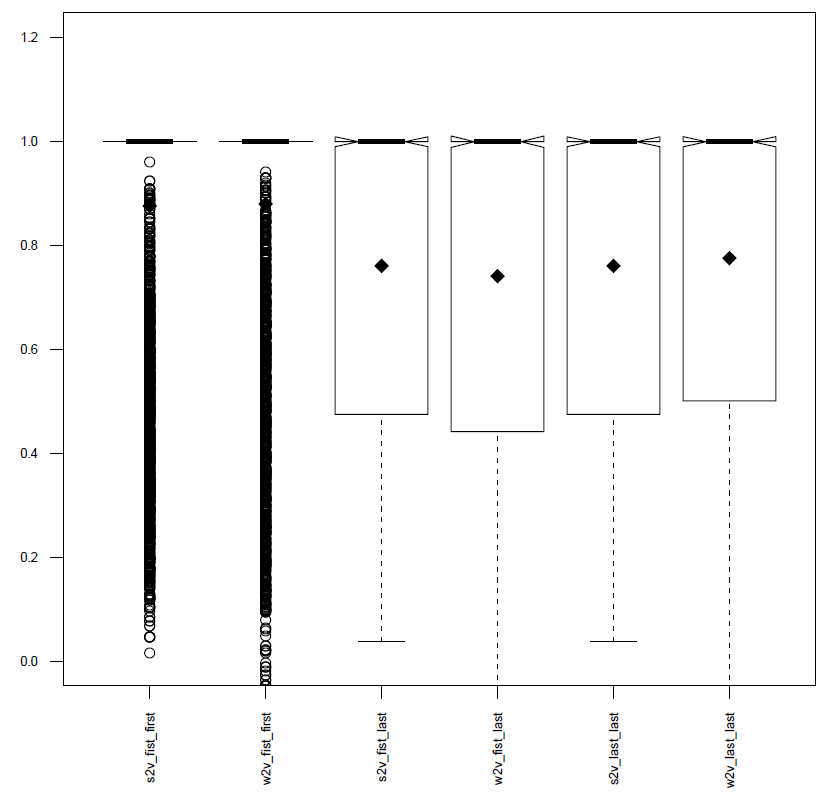
\includegraphics[width=\textwidth]{images/wordnet_nouns.PNG}
  \caption{Synset Comparison Nouns}
  \label{fig:wordnet_nouns}
\end{figure}

\noindent
In the figure \ref{fig:wordnet_nouns} the majority of the time the first word in the first sysnet is the word supplied itself, resulting in a similarity score of 1. The median values for both Sense2Vec (blue) and Word2Vec (purple) tend to be similar in figure \ref{fig:wordnet_nouns} However the outlier tails tend to be longer with Word2Vec.

\begin{figure}[H]
\centering
  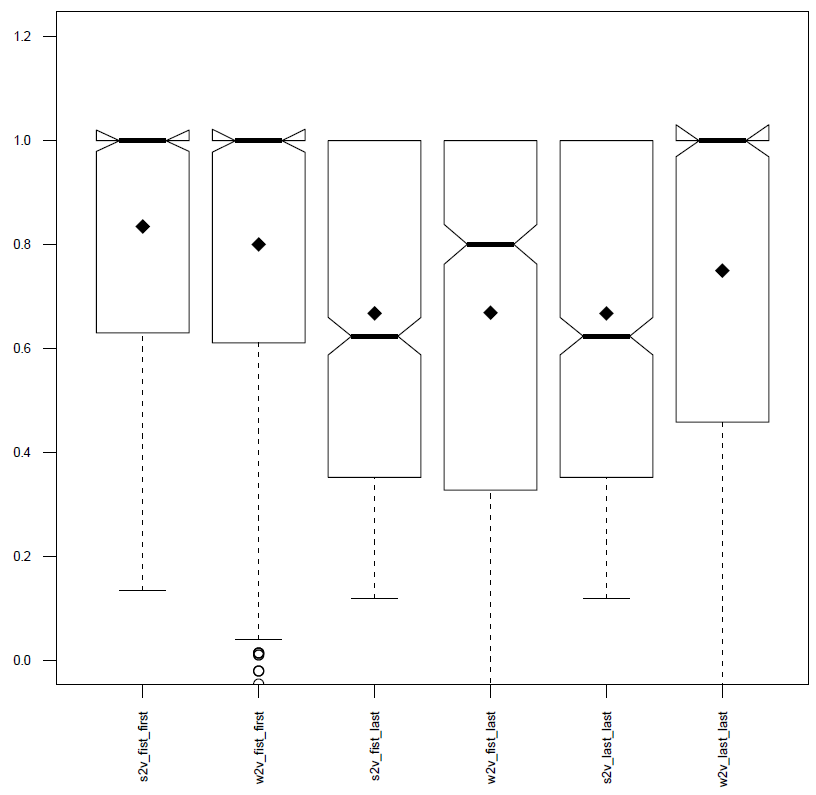
\includegraphics[width=\textwidth]{images/wordnet_verbs.PNG}
  \caption{Synset Comparison Verbs}
  \label{fig:wordnet_verbs}
\end{figure}

\noindent
Looking at the analysis of verbs in figure \ref{fig:wordnet_verbs} once again the tail of outliers and the max value for Word2Vec is higher. There is a high positive skew in the first two plots again due to the high number of exact matches. However Word2Vec for the rest of the groups has a large positive skew towards 1. With Sense2Vec the similarity drops with a slight negative skew which is expected as we progress further down and across the synsets.

With the above two plots \ref{fig:wordnet_verbs} and \ref{fig:wordnet_nouns} no median lies outside of Q1 or Q3 so it can not be said with confidence that the two methods are unique. However due to the high concentration of exact matches, the resulting data is left to be treated as outliers and pushed outside of Q3.

\section{Bloom's Taxonomy}
To attempt to show clear distinction between the two methods further analysis was completed using Bloom's Taxonomy as a basis. Similarity values are obtained between each verb in each level of the taxonomy excluding the verb itself ($n^2-n$ comparisons for each category). The verb was supplied to Word2Vec as is and tagged with the VERB POS tag for Sense2Vec, each level in the taxonomy was given its own boxplot.

\begin{figure}[H]
\centering
  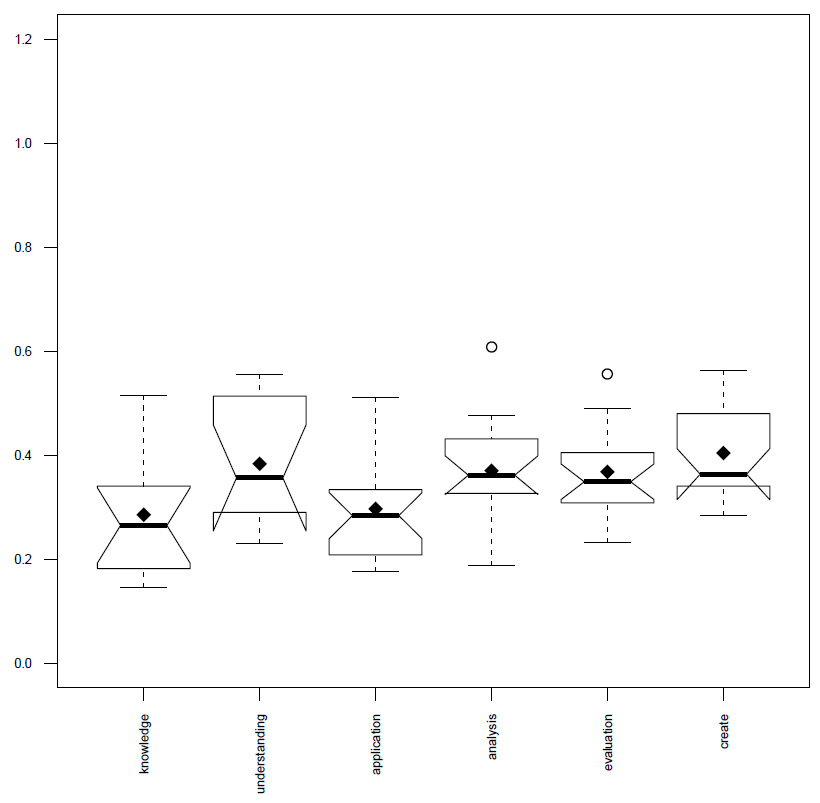
\includegraphics[width=\textwidth]{images/s2v_bloom.PNG}
  \caption{Sense2Vec Bloom's Taxonomy}
  \label{fig:bloom_s2v}
\end{figure}

\noindent
For Sense2Vec in figure \ref{fig:bloom_s2v} all levels form a condensed interquartile range with few outliers. In the lower 3 levels; create, evaluation and analysis the median of each lies within the interquartile range of the next showing there is a consistency in similarity score across the categories.

\begin{figure}[H]
\centering
  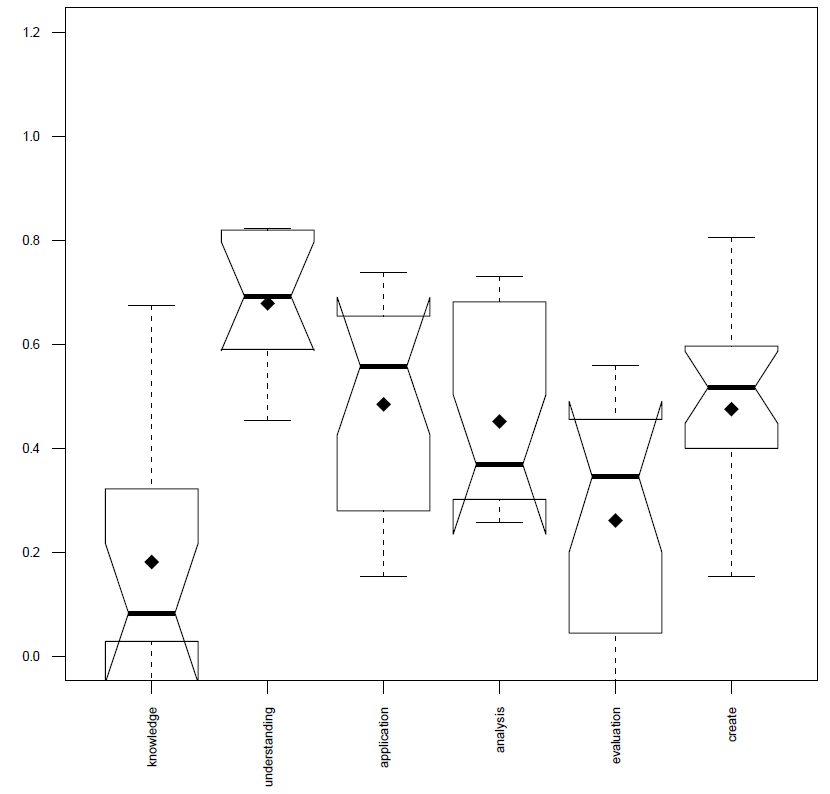
\includegraphics[width=\textwidth]{images/w2v_bloom.PNG}
  \caption{Word2Vec Bloom's Taxonomy}
  \label{fig:bloom_w2v}
\end{figure}

\noindent
When looking at Word2Vec in figure \ref{fig:bloom_w2v} the interquartile range is much less condensed and with the create category much more values are found outside the interquartile range. The median of the knowledge category lies well outside the interquartile range of the next category understanding, showing a lack of consistency of similarity score across the levels. While the median of the plots for Word2Vec is closer to 1 in two levels (understanding and create) and positively skewed towards 1 in two others (application and evaluation), this is negated by the lack of consistency across the levels with Word2Vec producing a low interquartile range for the knowledge and evaluation levels.

\begin{figure}[H]
\centering
\begin{minipage}{.5\textwidth}
  \centering
  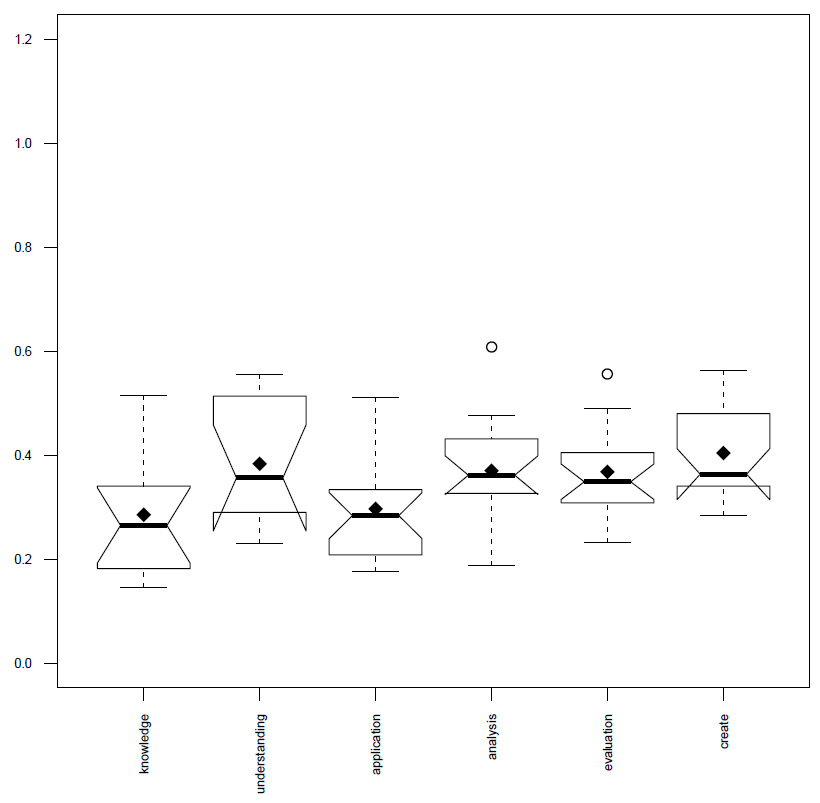
\includegraphics[width=1\linewidth]{images/s2v_bloom.PNG}
  \caption{(a) Sense2Vec}
  \label{fig:s2v}
\end{minipage}%
\begin{minipage}{.5\textwidth}
  \centering
  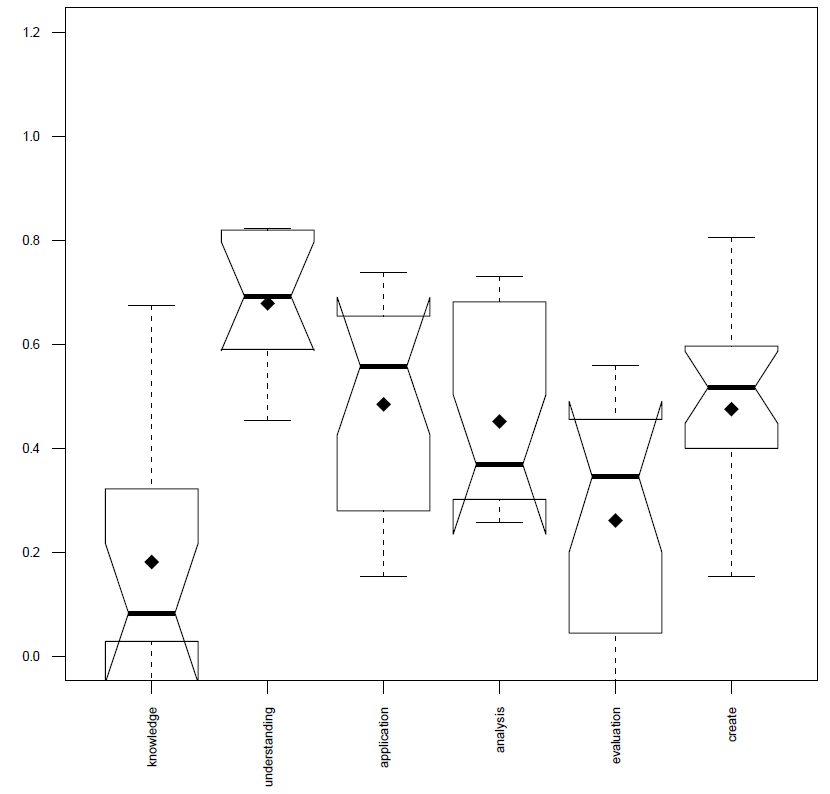
\includegraphics[width=1\linewidth]{images/w2v_bloom.PNG}
  \caption{(b) Word2Vec}
  \label{fig:w2v}
\end{minipage}
\caption{Side By Side Comparison}
\label{fig:side_by_side}
\end{figure}

\noindent
Finally looking the side by side comparison in figure \ref{fig:side_by_side} some distinction can be made between the two methods. For all levels except analysis and understanding the median in figure \ref{fig:w2v} is well outside the interquartile range and in some cases the max value of the corresponding level in figure \ref{fig:s2v}. Sense2Vec appears to show a more consistent similarity score across the six levels, Word2Vec's similarity score tends to fluctuate dramatically with a large difference between the first two levels on the plot in figure \ref{fig:w2v}. Also of note is the max value of both methods, for Sense2Vec the max and mix values are much smaller with fewer values outside the interquartile range. With Word2Vec the opposite is true not only is the interquartile range spread over a larger range of values but also the values outside this range extend further than that of Sense2Vec.

\begin{table}[H]
\centering
\begin{tabular}{|l|r|l|r|}
\hline
\multicolumn{2}{|c|}{Sense2Vec} & \multicolumn{2}{c|}{Word2Vec}   \\ \hline
List : List       & 1.0         & List : List      & 1.0          \\ \hline
List : Describe   & 0.31348008  & List : Describe  & -0.021850454 \\ \hline
List : Apply      & 0.26178     & List : Apply     & 0.06479468   \\ \hline
List : Compare    & 0.36929193  & List : Compare   & 0.0019651854 \\ \hline
List : Argue      & 0.2974751   & List : Argue     & -0.057712294 \\ \hline
List : Construct  & 0.18598314  & List : Construct & -0.057712294 \\ \hline
\end{tabular}
\caption{Comparison Across Categories}
\label{head_head_comp}
\end{table}

\noindent
In table \ref{head_head_comp} the head word of the first level is compared to the head word in each other level. Sense2Vec finds more similarity across levels and shows a general decline in similarity as the comparison progresses down the levels of the taxonomy. Word2Vec shows almost no relation between words across levels and no decline in similarity as the comparison proceeds down the levels. A full list of the verbs on each level of the taxonomy and the names of each category is located in Appendix F.

\chapter{Conclusion}
The task of extracting context and meaning from language is a difficult task and one which requires a large quantity of input data. Previous projects such as Word2Vec have achieved the goal of obtaining some context when producing word embeddings. However this process avoids a part of language which is integral to a words meaning, part of speech is an often overlooked semantic of language. The Sense2Vec project proposes a solution to include part of speech tagging in the training process for producing word embeddings. Upon investigating the use of this tagging in word embeddings some major advantages however this process is not without its drawbacks.

The most noteworthy advantage of this process is the reduction of confusion when investigating the use of a word that may have multiple parts of speech. The ability to specify more meaning for a specific word not only improves the accuracy by removing unwanted word embeddings not relevant to the word used in this context, it also separates clusters that would otherwise be combined had they not be separated by part of speech. Within section 4.3 Collisions three examples of this scenario were presented with Word2Vec providing a combination of words related to both the noun and verb form of the word. When compared to tagging the word; Sense2Vec provided greater context and allowed for clear separation between both forms of the word in all three cases. It was possible to make a clear distinction between the two word embedding systems using the WordNet project and Bloom's Taxonomy as baselines.

This process does not come without some caveats however, with the separation of word embeddings based on their part of speech the resulting vocabulary size is larger despite technically containing the same number of unique words. This also introduces a loss in context as the surrounding words will now be linked to the specific form of the word in that context, based on if it is used as a noun, verb adjective etc. All this requires a larger corpus of text with greater a diversity of words used in different forms, compare this to Word2Vec which can obtain a reasonable level of context based on a smaller corpus. Of course Sense2Vec also requires the corpus to be part of speech tagged before the training process begins a lengthy process and the most complex problem to solve. However once this is complete the training process is significantly quicker and the model produced is over four times smaller than that of Word2Vec, this is helped by the use of the GloVe library used to produce the model.



\bibliography{Thesis.bib} 
\bibliographystyle{ieeetr}

\chapter*{Acknowledgements}
I’d like to extend my gratitude to my supervisor Dr Diarmuid O'Donoghue, for first introducing the idea and providing help and guidance whenever needed. I am grateful for the work done by the Sense2Vec team and the provided documentation for their project. Also of course all friends and family who provided helpful input and suggestions throughout the project.

\section*{COVID-19}
On the 13th of March 2020 the University closed due to a government recommendation because of the COVID-19 pandemic. Almost all code to produce results for the project was completed by this stage, however only provisional results were logged at this time. The following week on the 20th of March all students were instructed to study and complete their work form home, at this time the two models used in this project were stored on an external hard drive for producing results at a later stage. However a few days later when running the code to produce the results it was found that combined; the models were approximately 8GB and once loaded into memory would exceed the RAM capacity of the available home PC. It was decided to migrate the processing of the results to Google Cloud, this process required two extra days of work to get the systems in place including uploading the models and creating new Python environments.

\end{document}
